\documentclass{article}
\usepackage[utf8]{inputenc}
\usepackage{graphicx}
	\DeclareGraphicsExtensions{.png, .jpeg}
\usepackage{caption}
% \usepackage{subcaption}
\usepackage[top=1in, bottom=1in, left=1in, right=1in]{geometry}

\title{Database Design and Implementation \\ HW 07}
\author{\underline{Team 08}\\Henriod, Terence\\Santoyo, Jorge \\Singh, Raja}
\date{\today}

\begin{document}

\clearpage
\maketitle
\thispagestyle{empty} % removes the page number from the title page

\begin{abstract} % Do we want to change this?
Create a logical ERD for each of the problems below using the crowsfoot format discussed in class. Be sure that each entity has the entity name at the top of the box, the primary key attribute or attributes in the middle of the box, and the non-key attributes in the bottom of the box. Lines should separate each part of the entity box. The ERD should not have any M:N relationships and all attributes should be placed within an entity. Each entity must have a primary key defined. A primary key may consist of one or more attributes. Each relationship should have at least one relationship verb or verb phrase. Please include all required foreign keys and denote the foreign key(s) with the notation (FK) on the ERD. \\
I recommend that you NOT use Visio for this assignment, but if you want to use Visio, then feel free to use it.
\end{abstract}
%
%
\newpage
\section{Exercise 01: Video-by-Mail Company}

Create a database for a company that delivers videos via mail to customers (a company such as Netflix). This database should keep track of the data required in the columns shown in the Excel Workbook ``MailVideoData-s15.xlsx". The worksheet in this workbook (VideoList) contains the data stored for customers’ video list – also called a ``queue". The video list contains videos that customers want to receive, have received, or have already received and returned. Sample data is provided in the worksheet to help you understand what needs to be stored for this application. The sample data is limited – the company has millions of customers, and each customer has at least 20 videos in his/her queue at any point in time. A customer can be of only one customer type at a time. Here is some additional information about the application:

\begin{itemize}
  \item A customer creates a queue to keep track of what videos he/she wants to receive in the mail. Most customers have 20-30 videos in their queue at any point in time.

  \item The data values for the ``status" of a video in the queue for a given customer can be as follows:
    \begin{itemize}
      \item \textbf{Queue}: A video is prioritized and waiting in the customer queue until it moves up the queue and is ready to be sent by the company. Each video that has a status of ``queue" must have a number attached. For example, a video for a customer that has a status of ``Queue-1" means that it is the first video in the queue.

      \item \textbf{Returned}: A video has been sent to the customer and was returned by the customer.

      \item \textbf{Home}: A video that is currently in the possession of a customer. A customer may keep a video as long as he/she wants, but customers are only allowed a pre-determined number of videos. This database does not keep track of how many videos a customer is allowed to keep at home; this database only keeps track of the status of videos in a customer’s list of videos.

      \item \textbf{Saved}: A video that is not yet released and available for customer use is tracked with a status of ``Saved". Any saved videos must be prioritized with a number. For example, a video with a status of ``Saved-2" means that it is the second video in the ``Saved" category for that customer. For example, Customer ID 7855 in the sample data has ``Scandal – Season 4" in queue with the status of ``Saved-2".
  \end{itemize}

  \item Data in the sample worksheet labeled as ``null" means that the data was not available at that time due to the status of the video. ``Null" data is non-existent. For example, the status of the video ``Divergent" for customerID 1234 indicates that the video is third in the queue waiting to be sent to the customer. Thus, the movie has not yet been sent or returned, so the date that the movie was sent does not exist and the date that it was returned does not exist.

  \item Assume each video has only one video category.

  \item Assume that there is a group of pre-defined video categories that must be stored in the database.

  \item Assume that a customer video rating is numeric and can go from 0 to 5 with a single digit after the decimal point. Assume that it is possible to calculate an average video rating from data in the database.

  \item Assume that it is possible for a customer’s video rating to be non-existent (null). A customer must enter his/her rating for a particular video. A customer is allowed to enter a video rating for a movie only once – there is no time dependent data for a video rating – so if a customer enters a new rating it is an “update” operation rather than an ``insert" operation.
\end{itemize}

\emph{Remember that it is not your job to design any processing for this system.} It is not your job to figure out how many videos a customer can have in his/her possession and ensure that the customer has only that quantity of videos. It is not your job to move videos in status from ``saved" to ``queue" when a video becomes available. Your job is to figure out how to store the data with a design that does not contain redundant data. Just design the data storage blueprint. \\

\begin{figure}[h!]
  \centering
  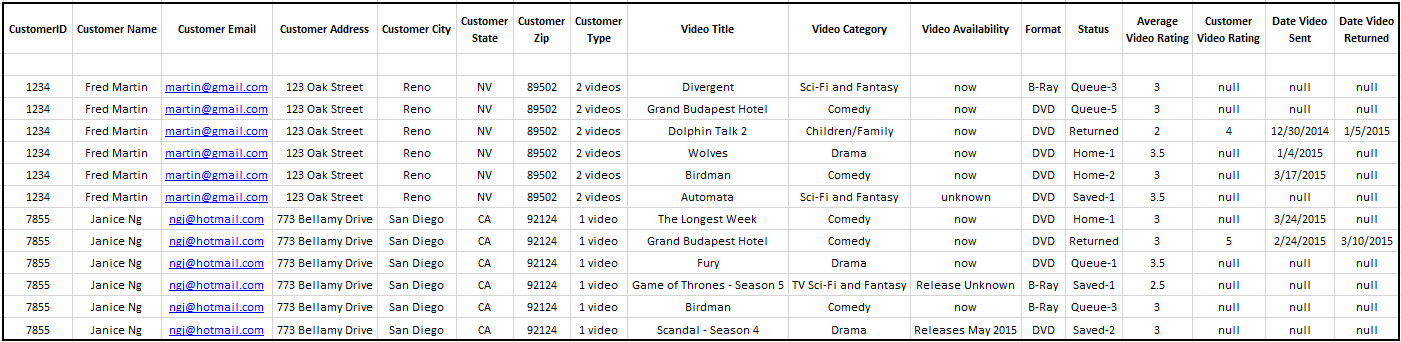
\includegraphics[width=.95\linewidth]{HW07_Exercise01_sample_data}
  \caption{The sample data for the exercise provided in MailVideoData-s15.xlsx.}
  \label{fig:HW07_Ex01_sample_data}
\end{figure}

\newpage
\textit{Solution}:\\

  \begin{figure}[h]
    \centering
    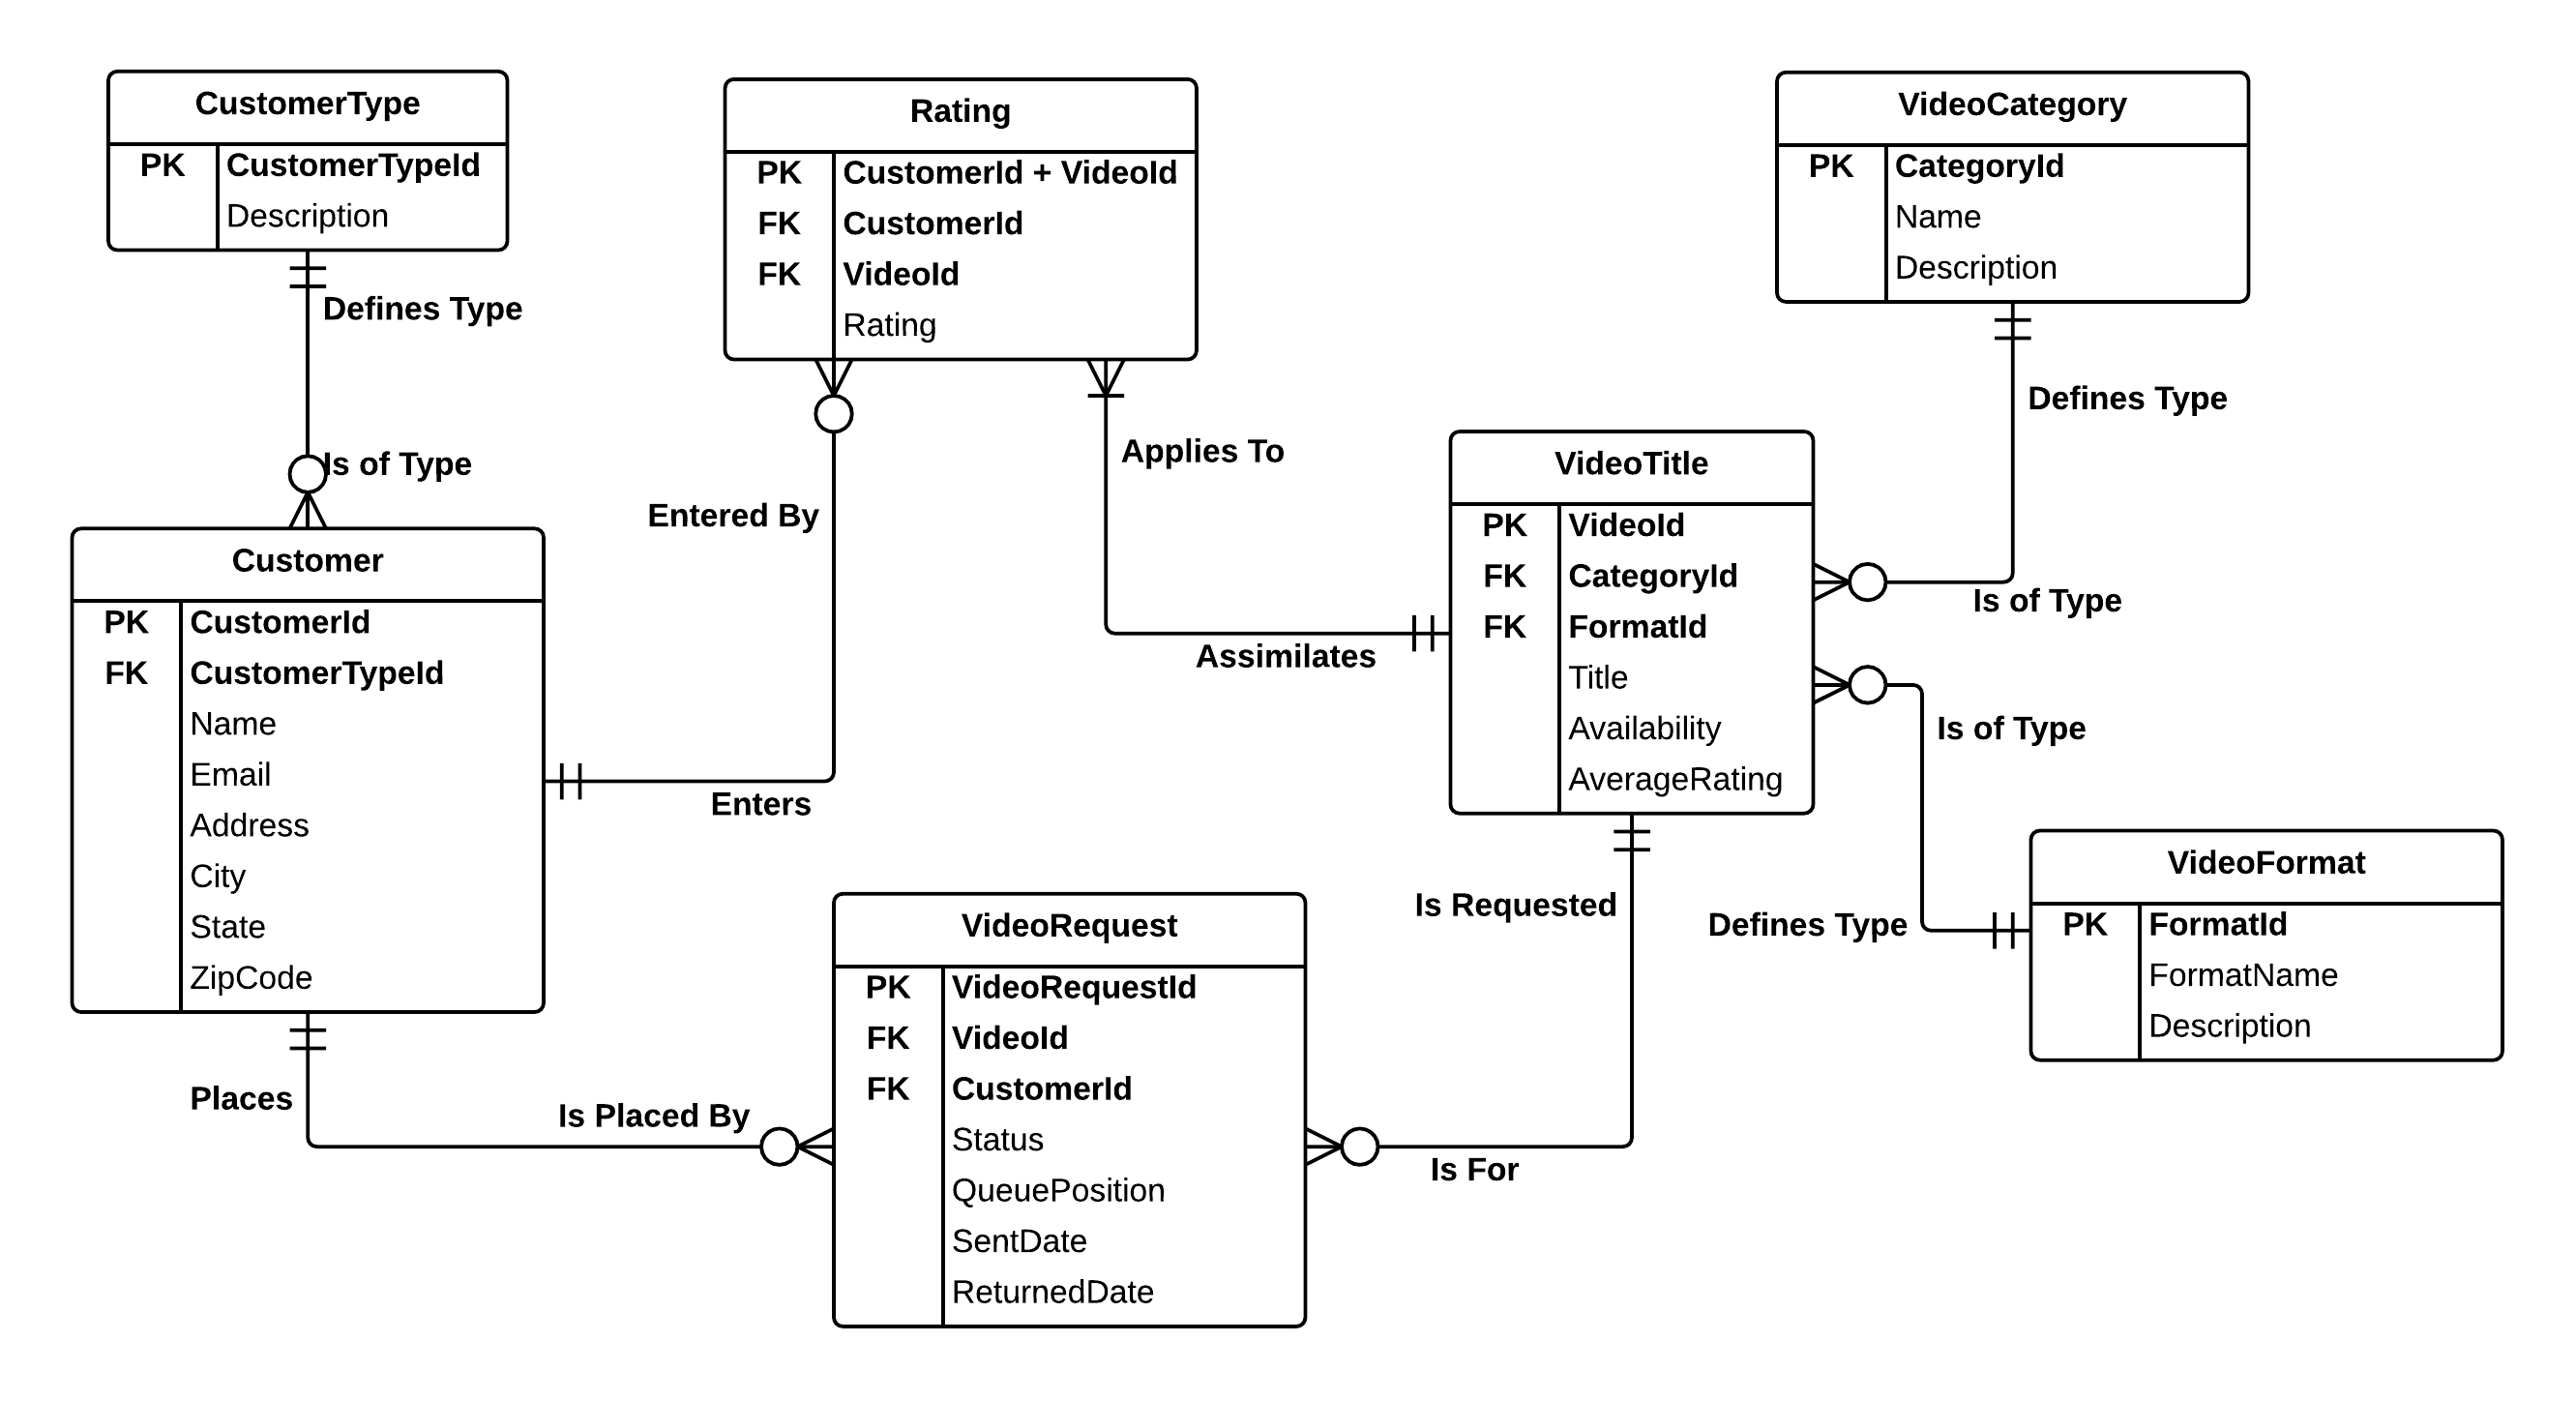
\includegraphics[width=.95\linewidth]{HW07_Exercise01_ERD}
    \caption{The solution ERD for the video-by-mail company's database.}
    \label{fig:HW07_Ex01}
  \end{figure}
%
%
\newpage
\section{Exercise 02: Business Graduate Placement}

The database will support the placement office of a leading graduate school of business. The primary purpose of the database is to schedule interviews and facilitate searches by students and companies. Here is additional information about the data to be stored:

\begin{itemize}
  \item Student data include a unique student identifier, a name, a phone number, and an email address.

  \item The placement office maintains a standard list of positions based on the Department of Labor’s list of occupations. Position data include a unique position identifier and a position description. Examples of position descriptions are: “Systems analyst,” “network systems administrator,” “sales – computer equipment,” “marketing analyst,” and “entry-level accountant.” These are standard descriptions that could be downloaded from the Department of Labor into the database for the placement office.

  \item Data about companies who interview students through the placement office include a unique company identifier, and a company name. Each company must relate its open positions into the standard list of positions maintained by the placement office (downloaded from the Department of Labor). For each open position, the company lists the city, state (or province/region) and country as well as the quantity of a specific type of position open in that city, state and country. For example, IBM might have the position of “sales – computer equipment” available in Dallas, Nashville, Washington DC, Paris, Perth, and Atlanta. In Dallas, IBM has a quantity of 2 of that position, while in Perth Australia, IBM has a quantity of 3 of that particular position available.

  \item The database must be able to generate a list of open positions for a given company and for all companies as well as a list of interviewers

  \item Interviewer data include a unique interviewer identifier, a name, a phone and an email address. Each interviewer works for only one company, but a company could have multiple interviewers.

  \item An interviewer may interview more than one student during a given day, but will only interview one student during a given interview.

  \item An interview includes a unique interview identifier, a date, a time, a location (building and room), one student and one interviewer. The length of an interview may vary in time. An interview may be with more than one interviewer. In other words, it is possible for two interviewers to meet with one student to conduct the interview. The database should be able to keep track of multiple interviewers for a single interview.

  \item An interview is not for a particular job. It is possible that an interviewer may interview a student for more than one job at the same time.

  \item The data will be used to create schedules for rooms, interviewers, companies, and students.
\end{itemize}

Keep in mind during your design that an entity almost always consists of more than one entity instance (in other words, it would be odd to have a table with only one row). For example, if you find yourself tempted to create an entity for the “placement office” then think about what data you will be storing in that entity. This organization has only one ``placement office" so there would be only one instance of that entity. An entity with only one instance isn’t really an entity. Also keep in mind that an ERD is not a process diagram. It doesn’t really matter who does what, such as how a student will be matched with an interviewer, or where the data comes from – you should focus on creating a blueprint of all data necessary to support the application. Finally, think about what the application is supposed to accomplish when designing the required data. Think about what output information (reports and queries) might need to be generated from the system to ensure that your entities are related in such a way that the output could be produced. \\

\newpage
\textit{Solution}:\\

  \begin{figure}[h!]
    \centering
    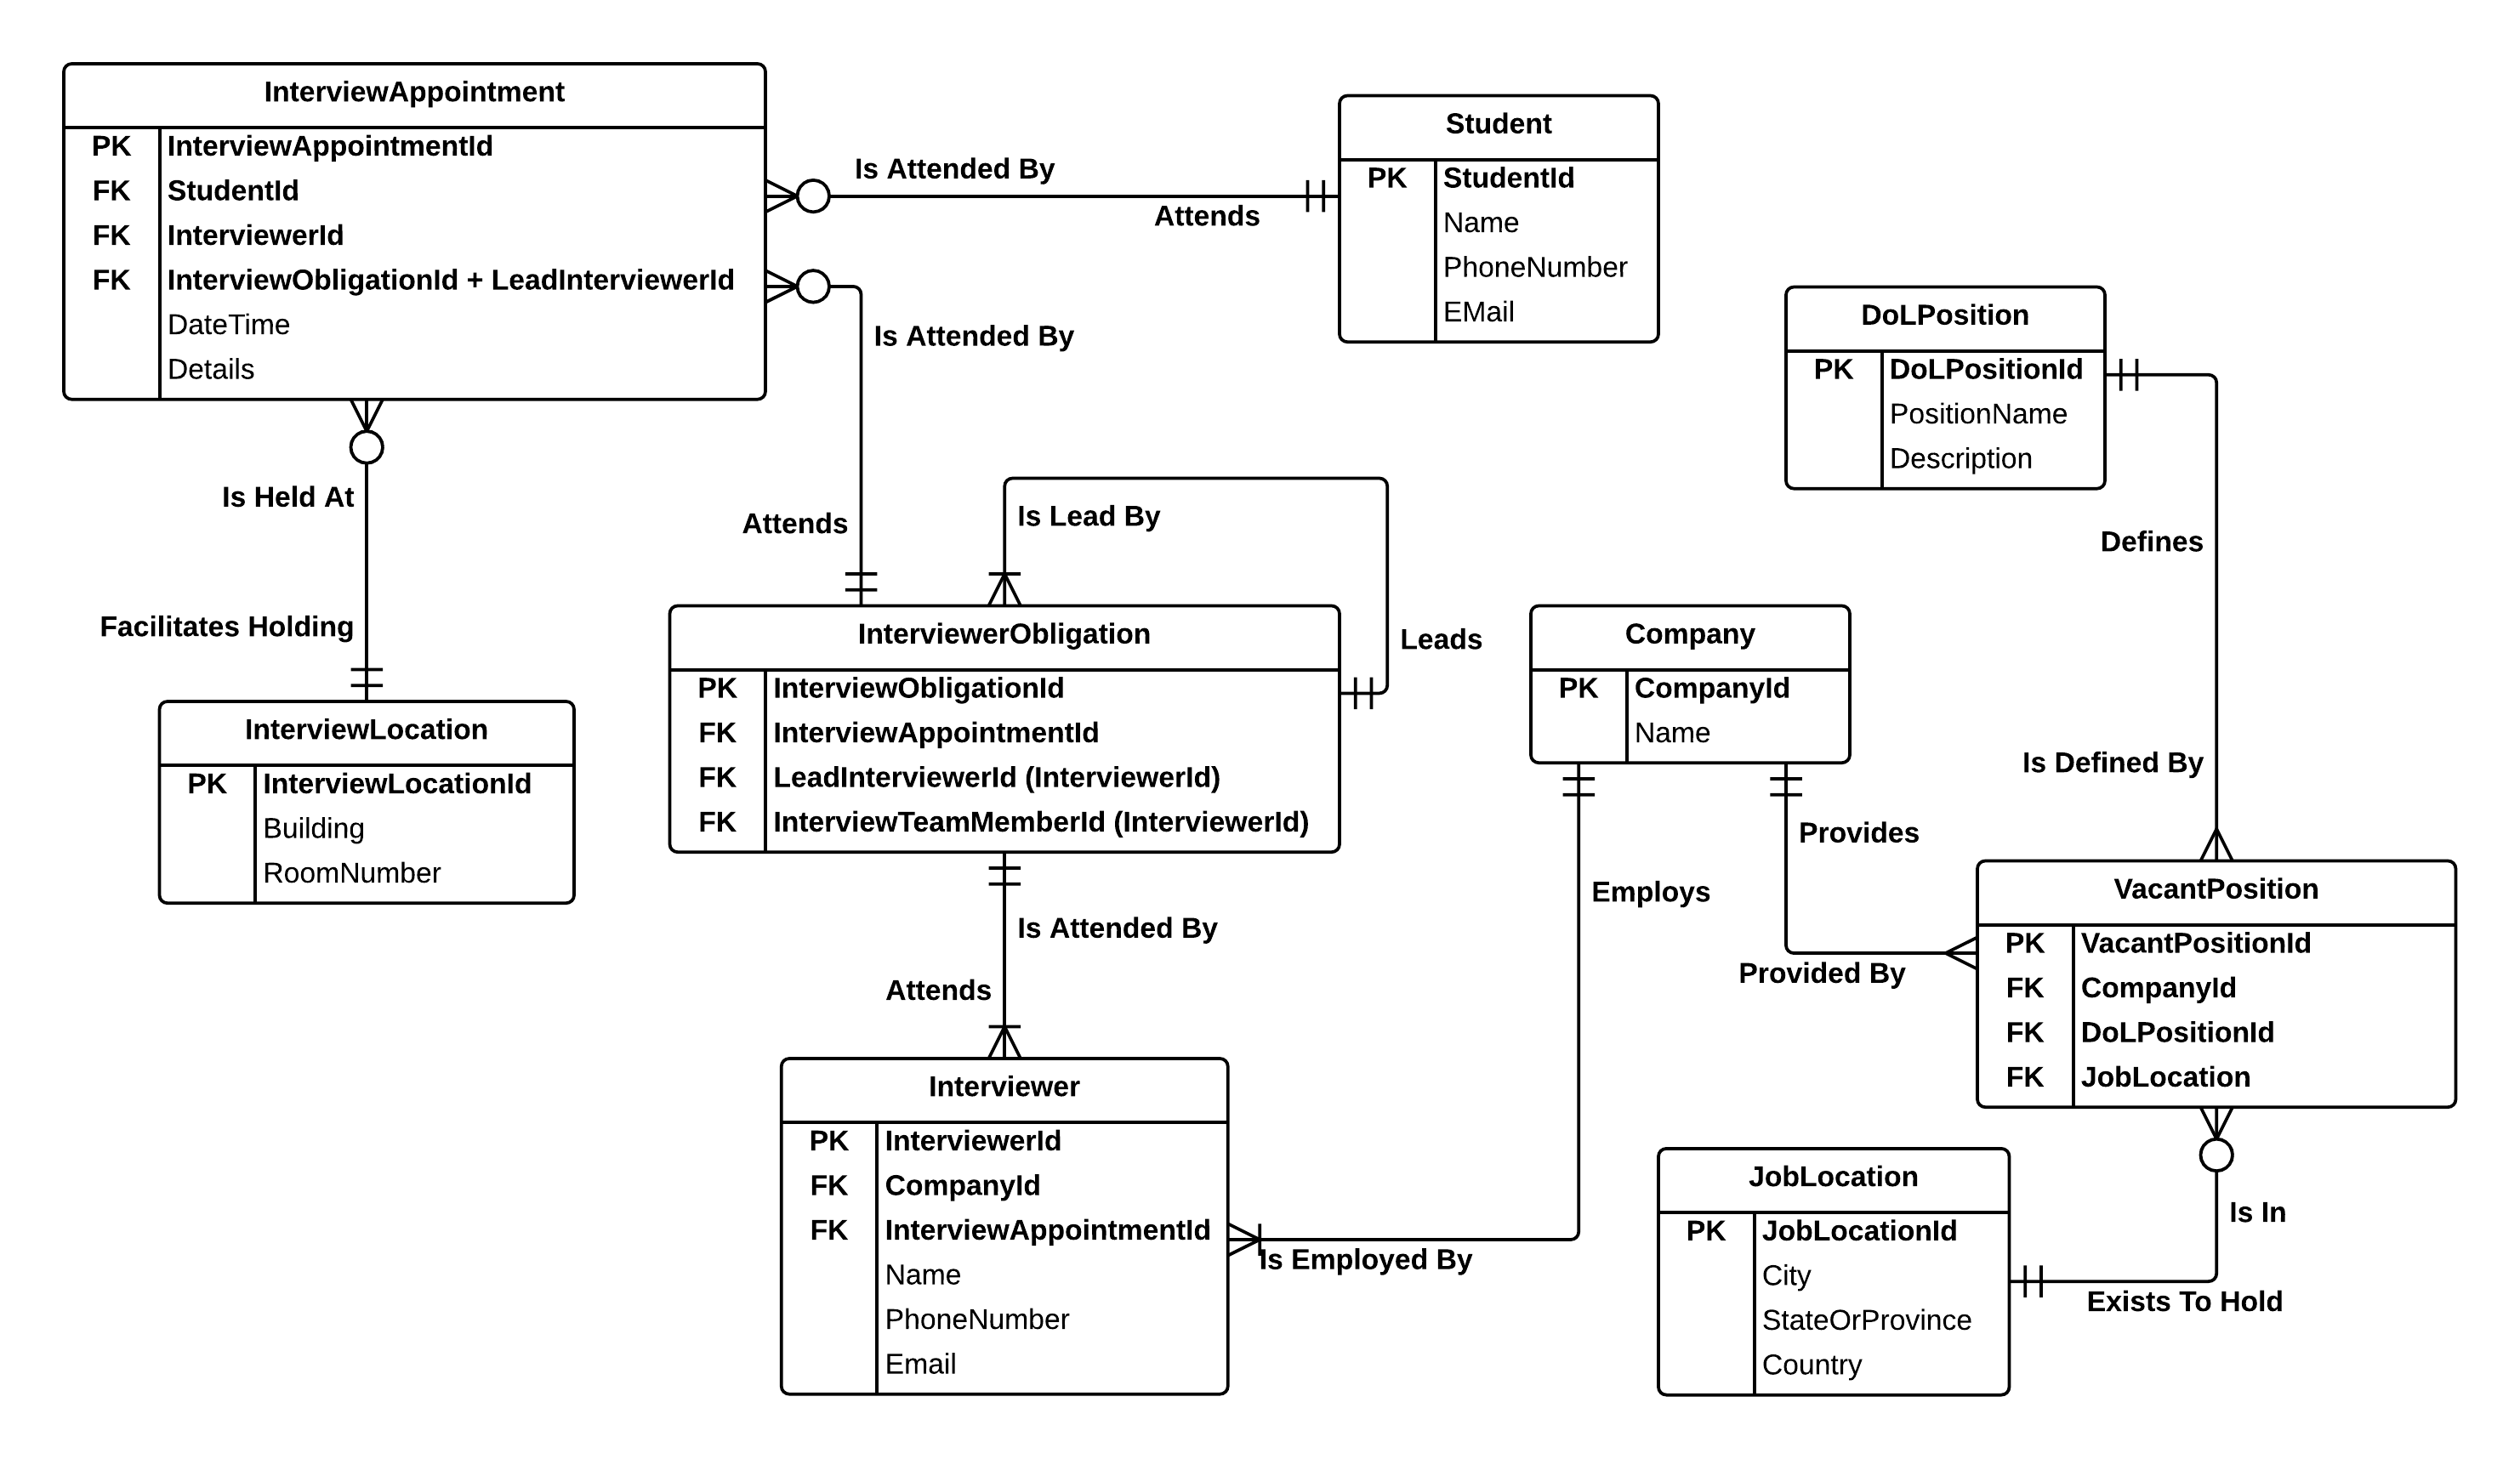
\includegraphics[width=.95\linewidth]{HW07_Exercise02_ERD}
    \caption{The solution ERD for the graduate job placement company's database.}
    \label{fig:HW07_Ex02}
  \end{figure}

Note: The directions posed an arrangement that was difficult to reason through: each interview should have one interviewer, but multiple interviewers could work on the same interview. In order to avoid what appeared to be a necessary many-to-many relationship (even though one of those manys might not be allowed), we created the idea of an ``Interviewer Obligation," which can be thought of as an appointment that an indivdual interviewer must keep. Using these, we attempt to form an interviewer team (like for a panel interview, or an interview process with stages), where one interviewer will be the lead interviwer. The concept of the lead interviewer allows each InterviewAppointment to have only one interviewer listed as an attribute. The interviewer team could take shape via an SQL query that joins \texttt{InterviewerObligation}s on \texttt{LeadInterviewerId}. If it helps, the concept of employees who may or may not manage other employees motivated our thinking for creating an entity with a unary relationship.

\end{document}